


\tikzset{every picture/.style={line width=0.75pt}} %set default line width to 0.75pt        

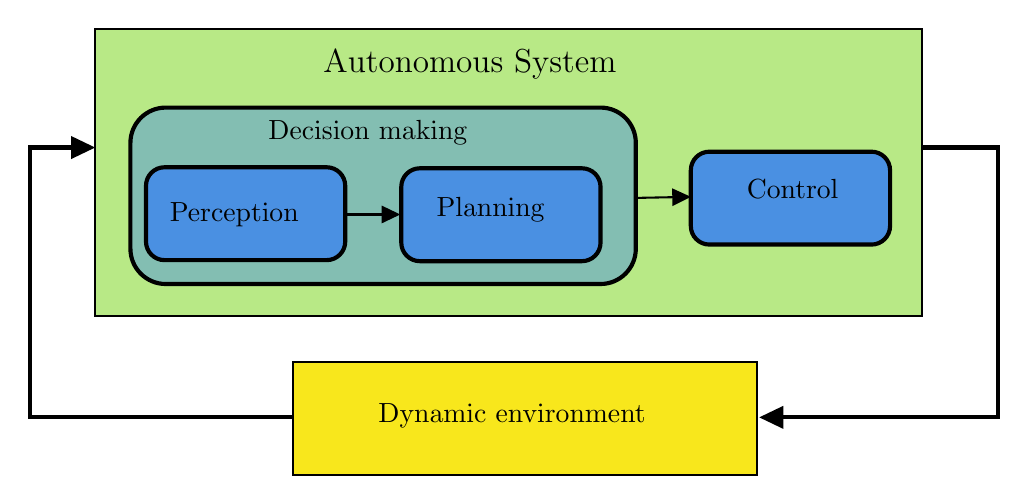
\begin{tikzpicture}[x=0.75pt,y=0.75pt,yscale=-1,xscale=1]
	%uncomment if require: \path (0,300); %set diagram left start at 0, and has height of 300
	
	%Shape: Rectangle [id:dp27957619560066704] 
	\draw  [fill={rgb, 255:red, 184; green, 233; blue, 134 }  ,fill opacity=1 ] (43,48.75) -- (441.5,48.75) -- (441.5,187.25) -- (43,187.25) -- cycle ;
	%Rounded Rect [id:dp7625981193027371] 
	\draw  [color={rgb, 255:red, 0; green, 0; blue, 0 }  ,draw opacity=1 ][fill={rgb, 255:red, 74; green, 144; blue, 226 }  ,fill opacity=1 ][line width=1.5]  (330,116.95) .. controls (330,112.01) and (334.01,108) .. (338.95,108) -- (417.05,108) .. controls (421.99,108) and (426,112.01) .. (426,116.95) -- (426,143.8) .. controls (426,148.74) and (421.99,152.75) .. (417.05,152.75) -- (338.95,152.75) .. controls (334.01,152.75) and (330,148.74) .. (330,143.8) -- cycle ;
	%Straight Lines [id:da826125804046745] 
	\draw    (304.5,130.25) -- (327,129.81) ;
	\draw [shift={(330,129.75)}, rotate = 178.88] [fill={rgb, 255:red, 0; green, 0; blue, 0 }  ][line width=0.08]  [draw opacity=0] (8.93,-4.29) -- (0,0) -- (8.93,4.29) -- cycle    ;
	%Rounded Rect [id:dp7912077043288683] 
	\draw  [color={rgb, 255:red, 0; green, 0; blue, 0 }  ,draw opacity=1 ][fill={rgb, 255:red, 74; green, 144; blue, 226 }  ,fill opacity=0.48 ][line width=1.5]  (60,103.75) .. controls (60,94.36) and (67.61,86.75) .. (77,86.75) -- (286.5,86.75) .. controls (295.89,86.75) and (303.5,94.36) .. (303.5,103.75) -- (303.5,154.75) .. controls (303.5,164.14) and (295.89,171.75) .. (286.5,171.75) -- (77,171.75) .. controls (67.61,171.75) and (60,164.14) .. (60,154.75) -- cycle ;
	%Rounded Rect [id:dp050693216378291606] 
	\draw  [color={rgb, 255:red, 0; green, 0; blue, 0 }  ,draw opacity=1 ][fill={rgb, 255:red, 74; green, 144; blue, 226 }  ,fill opacity=1 ][line width=1.5]  (67.5,124.45) .. controls (67.5,119.51) and (71.51,115.5) .. (76.45,115.5) -- (154.55,115.5) .. controls (159.49,115.5) and (163.5,119.51) .. (163.5,124.45) -- (163.5,151.3) .. controls (163.5,156.24) and (159.49,160.25) .. (154.55,160.25) -- (76.45,160.25) .. controls (71.51,160.25) and (67.5,156.24) .. (67.5,151.3) -- cycle ;
	%Rounded Rect [id:dp6167247502432494] 
	\draw  [color={rgb, 255:red, 0; green, 0; blue, 0 }  ,draw opacity=1 ][fill={rgb, 255:red, 74; green, 144; blue, 226 }  ,fill opacity=1 ][line width=1.5]  (190.5,124.95) .. controls (190.5,120.01) and (194.51,116) .. (199.45,116) -- (277.55,116) .. controls (282.49,116) and (286.5,120.01) .. (286.5,124.95) -- (286.5,151.8) .. controls (286.5,156.74) and (282.49,160.75) .. (277.55,160.75) -- (199.45,160.75) .. controls (194.51,160.75) and (190.5,156.74) .. (190.5,151.8) -- cycle ;
	%Straight Lines [id:da3281578111728798] 
	\draw    (163.5,138.25) -- (179.5,138.25) -- (187,138.25) ;
	\draw [shift={(190,138.25)}, rotate = 180] [fill={rgb, 255:red, 0; green, 0; blue, 0 }  ][line width=0.08]  [draw opacity=0] (8.93,-4.29) -- (0,0) -- (8.93,4.29) -- cycle    ;
	%Shape: Rectangle [id:dp8888738733811714] 
	\draw  [fill={rgb, 255:red, 248; green, 231; blue, 28 }  ,fill opacity=1 ] (138.5,209.25) -- (362,209.25) -- (362,263.75) -- (138.5,263.75) -- cycle ;
	
	%Straight Lines [id:da14809135342937618] 
	\draw [line width=1.5]    (442,106) -- (478,106) -- (478,236) -- (367,236) ;
	\draw [shift={(363,236)}, rotate = 360] [fill={rgb, 255:red, 0; green, 0; blue, 0 }  ][line width=0.08]  [draw opacity=0] (11.61,-5.58) -- (0,0) -- (11.61,5.58) -- cycle    ;
	%Straight Lines [id:da5537882213887542] 
	\draw [line width=1.5]    (138,236) -- (11.5,236) -- (11.5,106) -- (39,106) ;
	\draw [shift={(43,106)}, rotate = 180] [fill={rgb, 255:red, 0; green, 0; blue, 0 }  ][line width=0.08]  [draw opacity=0] (11.61,-5.58) -- (0,0) -- (11.61,5.58) -- cycle    ;
	
	% Text Node
	\draw (151.5,57.5) node [anchor=north west][inner sep=0.75pt]   [align=left] {{\large Autonomous System}};
	% Text Node
	\draw (77.5,131) node [anchor=north west][inner sep=0.75pt]   [align=left] {Perception};
	% Text Node
	\draw (206,128.5) node [anchor=north west][inner sep=0.75pt]   [align=left] {Planning};
	% Text Node
	\draw (355.5,120) node [anchor=north west][inner sep=0.75pt]   [align=left] {Control};
	% Text Node
	\draw (125,91.5) node [anchor=north west][inner sep=0.75pt]   [align=left] {Decision making};
	% Text Node
	\draw (178,228) node [anchor=north west][inner sep=0.75pt]   [align=left] {Dynamic environment};
	
	
\end{tikzpicture}